\section{Real Time Communication and Adaptive Bitrate Streaming}\label{sec:rt_and_adaptive_bitrate_streaming}

Whenever we look at different types of streaming, it is important to consider the 
different requirements that come with them.
We differentiate between a one-sided communication, where an increase in delay 
in order to gain a higher quality is acceptable, and a two-sided communication, 
where a low delay is crucial for a satisfactory user experience.
The former allows for more complex setups like the one considered 
in~\autoref{subsec:adaptive_bitrate_streaming} while the latter requires
a more direct approach which will be discussed in the following subsection.

\subsection{Real Time Communication}
When looking at streaming setups that consider real-time constraints, such as conferencing 
where interhuman communication is involved, the objectives of the connection tend towards
low latency.
In order to provide natural-feeling human communication, the delay between the sender 
and the receiver has to be minimal.
This type of communication between devices is often referred to as ``Real-Time Communication'' 
(RTC) and used in many applications, such as Zoom, Skype, or Discord.

\subsubsection{Mechanisms and Ideas}
The main goal of such systems is to minimize the delay between the sender and the receiver
while additionally allowing all parties to communicate with each other.
A lot of design decisions are made with this in mind.
One design decision for a large conferencing system like Zoom
might consider the usage of peer-to-peer (P2P) connections versus a server-based
approach.
While P2P might allow for lower latencies in case of a small number of participants,
a server-based approach scales a lot better and can therefore provide a better
resource utilization.

\subsubsection{Implications on Streaming Setup}
The need for low latency also has implications for the fundamental setup.
An example of such an implication is the connection design between the 
real-time connection network (RTCN) and a client.
Since retransmissions are expensive in terms of latency, a setup should strive to minimize 
the distance a packet has to travel through an unreliable network.
This could be achieved by having multiple, strategically placed edge-servers.
Those would internally use a connection, which is more reliable compared to the internet.
Such a reliable connection would then be used for a large part of long-distance transmissions
(e.g.~intercontinental ones).
This way, packet loss occurring during the client-to-edge-server connection would not have a big 
impact on the overall latency of the connection.
A visualization of such an approach can be seen in~\autoref{fig:real-time-streaming-connections}.

\vspace{0.5cm}
\begin{figure}[H]
    \centering
    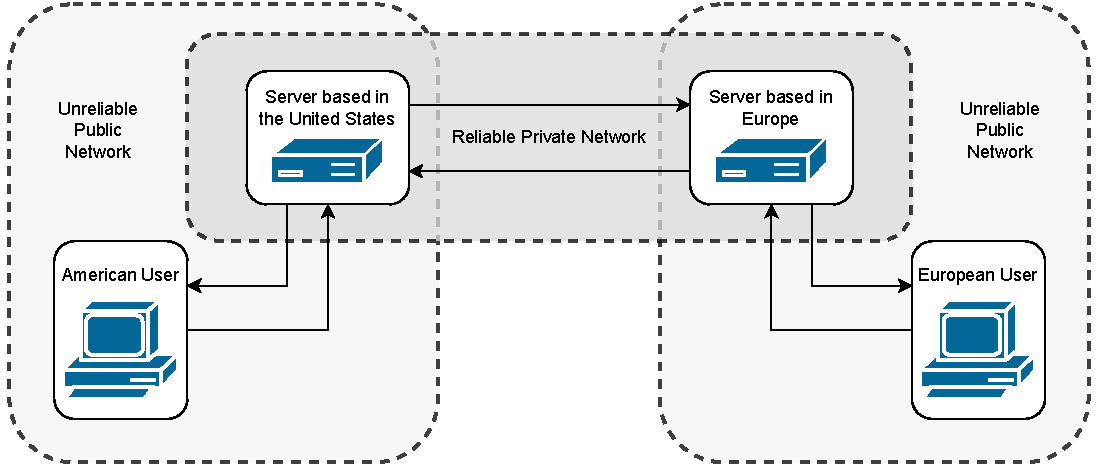
\includegraphics[width=0.8\textwidth]{figures/02_background/real-time-streaming-connections.drawio.pdf}
    \caption[Real-time streaming connections]{A setup with multiple edge servers worldwide can help minimize a connection's latency.}\label{fig:real-time-streaming-connections}
\end{figure}

\subsection{Adaptive Bitrate Streaming}\label{subsec:adaptive_bitrate_streaming}
Multimedia streaming is a big part of the internet, and many optimizations have
been developed to improve the quality of service for the end-users.
This includes considering (in real-time) parts of the clients' connection state, 
such as available bandwidth, and adapting the rate at which a server sends 
data~\parencite{cloudflare-what-is-adaptive-bitrate-streaming,imagekit-adaptive-bitrate-streaming}.
Such a process is called ``Adaptive Bitrate Streaming'' (ABS) and is employed in many 
of today's streaming setups~\parencite{netflix-optimizing-stream-experience}.

\vspace{0.5cm}
\begin{figure}[H]
    \centering
    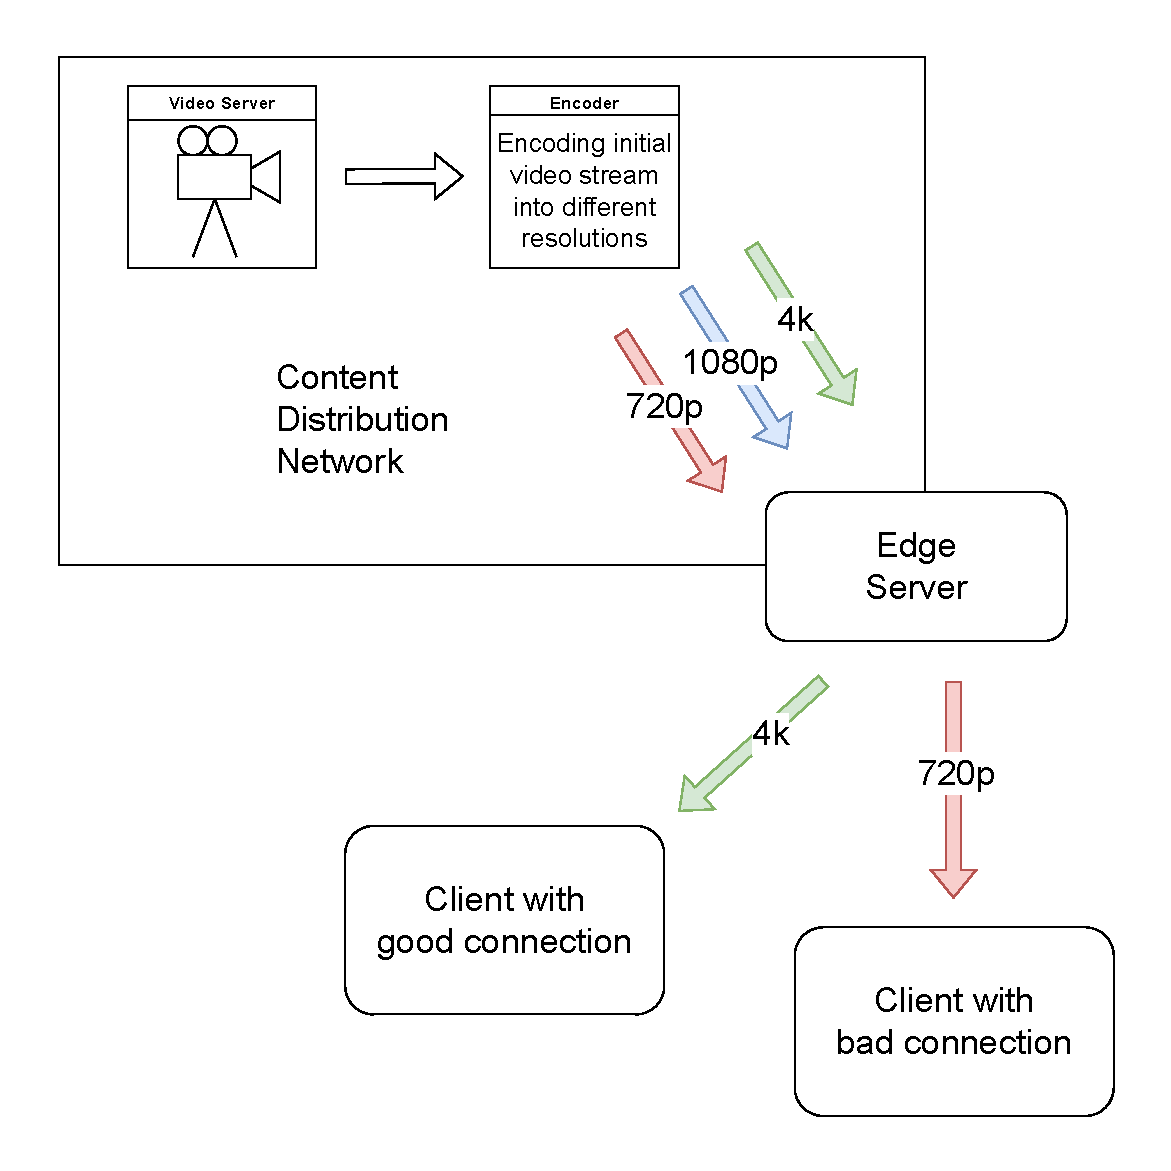
\includegraphics[width=\textwidth]{figures/02_background/adaptive-bitrate-streaming.drawio.pdf}
    \caption[Adaptive streaming schematic]{Behind the scenes, multiple streams with different
    resolutions exist to allow adapting to a user's bitrate.}\label{fig:adaptive-bitrate-streaming}
\end{figure}
% The way the example implementation of fast-realys in this thesis is set up,
% is that the video server will encode into each packet its priority.
% For example I-frames have a high priority while P-frames have a lower
% priority.
% The relay then can decide not to forward certain packets to a client if
% the client is experiencing congestion.
\vspace{1cm}

\subsubsection{Mechanisms and Ideas}
ABS implements the simple idea of changing the amount of data sent to a client 
based on the client's connection quality.
This means a client with a good connection gets a higher-quality stream than 
one with a bad connection.
For this, the internal setup needs to be able to provide multiple streams with
different resolutions and bitrates.
An example setup can be seen in~\autoref{fig:adaptive-bitrate-streaming} where
an encoder creates streams with different resolutions.
This allows an edge server, which manages the connections to the clients, 
to switch between those streams based on the connection state of a specific client.
Twitch and YouTube Live are examples where, although more complex, similar setups
are used to provide a better user experience.
The premise of such a setup is that in case of a bad connection, it is still 
preferable to be able to watch a stream continuously, even if that means
cutting down on quality.
However, one must keep 
the differences between Video-on-Demand (VoD) and live streaming in mind when looking at such real-world examples.
The latter might require more computation before a video is sent since the media 
has to be processed on the fly since it is created in real time.
For VoD, on the other hand, the media already exists in its final form. 

\subsubsection{Implications on Streaming Setup}
ABS forces a few changes to the way servers and relays are set up.
First, as~\autoref{fig:adaptive-bitrate-streaming} shows, there needs to 
be an ``encoding'' component that turns the single, high-quality stream  
received from the streaming source into multiple streams with different resolutions.
In some cases, the relay also needs to keep track of the clients' connection quality, e.g.~using 
measurements like RTT, packet loss, et cetera, and decide which stream to forward to the client.
In other cases, this can also be done by the client itself.
Since the connection quality can change dynamically, the one responsible for
the measurements must continuously monitor the connection and potentially trigger a change in 
the used stream.
The MoQ standard does not yet specify if the decision to adapt the bitrate lies with the
publisher or the subscriber.
Besides encoding and monitoring aspects, the system also has increased storage requirements
since stream data will essentially be duplicated.
